%# -*- coding: utf-8-unix -*-
%%==================================================
%% chapter0.tex for SJTU Master Thesis
%%==================================================


\chapter{智能温室的实践与应用}
\label{chapter:Application}
温室CFD仿真模型建立完成后,需要借助其进行各种计算,得出不同的计算结果并进行分析,才能发挥出数值仿真的价值和优势。智能温室监测与控制系统实现后之后,需要在实践应用中对其有效性、准确性、可靠性和稳定性进行验证。本章通过温室CFD仿真模型及其结果分析,得出了智能温室系统监测点位置选择优化方案、机械通风参数优化方案和机械通风控制策略优化方案。

\section{监测点位置选择与优化}
温室生产面积通常较大,一般在1200 $\text{m}^{2}$以上,为了能够有效监测温室整体的环境状态,监测系统通常需要布置大量密集的监测点和传感设备,从而导致监测硬件成本过高。因此,为了使用尽量少的监测点准确地反映温室整体的环境分布和变化,本文通过对温室CFD仿真模型的仿真结果进行分析,把握温室内环境的分布和变化规律,从而选择和优化智能温室系统的监测点位置。

不同的温室在不同的大环境下,室内环境分布差别很大,监测的关注点也有较大的差别,本文针对实验温室在夏季高温条件下需要机械通风的情况下的监测为例进行监测点的优化,其它温室和环境下,可以充分利用无线传感器的优势,对温室环境分布进行分析后优化监测点的位置。

农业生产主要关注植物冠层的空气温湿度分布和变化,因此空气温湿度监测点的位置首先可以确定在植物冠层,即截面L处。为了让监测系统更加有效地反映温室的整体环境状态,系统需要确定能够代表温室内平均水平的监测点,如图\ref{fig:TL}所示,温室第3栋受温室推拉门的影响空气温度明显高于其它区域,因此该区域内可以用来监测温室内的最高气温阈值,如果无需监测最高气温的话,该区域不适宜作为空气温湿度监测点;靠近湿帘和风机的位置由于通风时空气流动剧烈,容易对空气温湿度监测点产生较大的影响,因此也不适宜作为空气温湿度监测点;温室第1、2、4、5栋的中间位置空气温度分布较为均匀且空气流动较温和,本文认为较为适宜作为空气监测点。

对于土壤温湿度状态的监测,由于土壤的温湿度一般情况下分布均匀且变化缓慢,所以要求较低,选取温室的中心位置进行监测即可。对于光照强度的监测,只要不被温室内的作物或其它障碍物遮挡即可。

综合考虑,针对实验温室在夏季高温条件下需要机械通风情况下的监测,本系统选取第1、2、3、4、5栋的中间位置的植物冠层位置作为空气温湿度监测点,选取温室中心位置作为土壤温湿度和光照强度的监测点。此时,可以仅使用最少5个监测点即可获取温室内环境状态的整体平均分布和变化,有效地减少了监测点的布置数量和布置密集度,从而有效地降低了系统的监测成本。

\section{智能温室远程监测与控制系统应用}
本文设计并实现的基于农业物联网的智能温室监测与控制系统在实验温室,即上海市崇明区连栋塑料温室(东经121.74,北纬31.50),进行了实施运行。协调器如图\ref{fig:real:a}所示,路由器节点封装如图\ref{fig:real:b}所示,终端节点封装如图\ref{fig:real:c}所示。

\begin{figure}[!htbp]
	\centering
    \subfigure[协调器]{
		\label{fig:real:a} 
		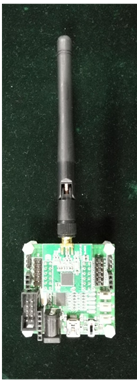
\includegraphics[height=4cm]{real/Cor.png}
	}
    \subfigure[路由器]{
		\label{fig:real:b} 
		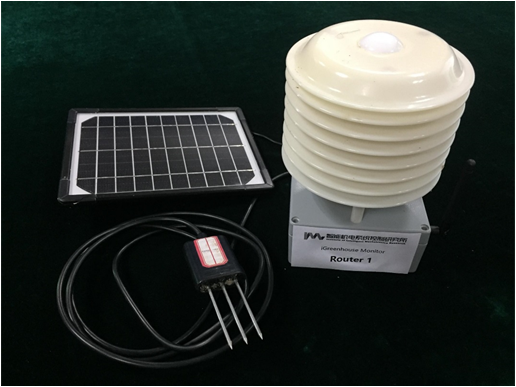
\includegraphics[height=4cm]{real/Router.png}
	}
	\subfigure[终端节点]{
		\label{fig:real:c}
		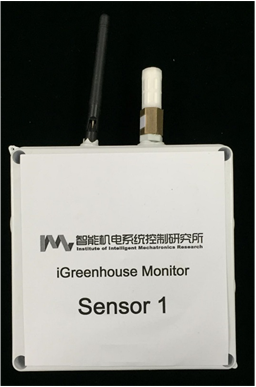
\includegraphics[height=4cm]{real/Node.png}
	}
    \bicaption[fig:real]{协调器、路由器封装和终端节点封装}{协调器、路由器封装和终端节点封装}{Fig}{Coordinator, router and endnode}
\end{figure}
根据通过仿真模型得到的温室监测点位置的优化结果,系统确定温室监测点布置方案:在实验温室内第1、2、4、5栋的中间位置各布置一个终端节点,用以监测温室内的空气温湿度分布和变化;在温室的中心位置布置一个路由器节点,用以监测温室内的土壤温湿度和光照强度,路由器节点还带有空气温湿度传感器,可以根据该节点的数据判断温室内最高温度的阈值,此外路由器节点还可以对无线传感器网络起到扩展的作用,从而能够监测更大范围内的温室,使距离较远的监测点能够接入网络,保证网络的覆盖范围和稳定性。此次实施运行,还在连栋塑料温室旁的9个单栋薄膜温室内各布置一个监测点,大部分为终端节点,少数为路由器节点,以保证网络的覆盖范围和稳定性。

系统运行期间运行稳定正常,无线传感器网络传输稳定可靠,温室内外数据采集准确正常,响应迅速,数据上传同步延迟在1s以内,控制指令下达准确迅速,延迟在5s以内,控制状态获取正常。数据中心工作正常,未发生慢查询或查询异常。云端WEB服务器及服务端程序运行稳定正常,接口响应迅速,数据返回完整准确。如图\ref{fig:snapshot}所示为Android平台上的终端程序截图,IOS平台和WEB页面显示完全相同,程序运行正常,数据获取与解析正常。现场图像采集设备工作正常,视频延时在10 s以内,显示正常如图\ref{fig:snapshot}所示。

	\begin{figure}[!htbp]
		\centering
		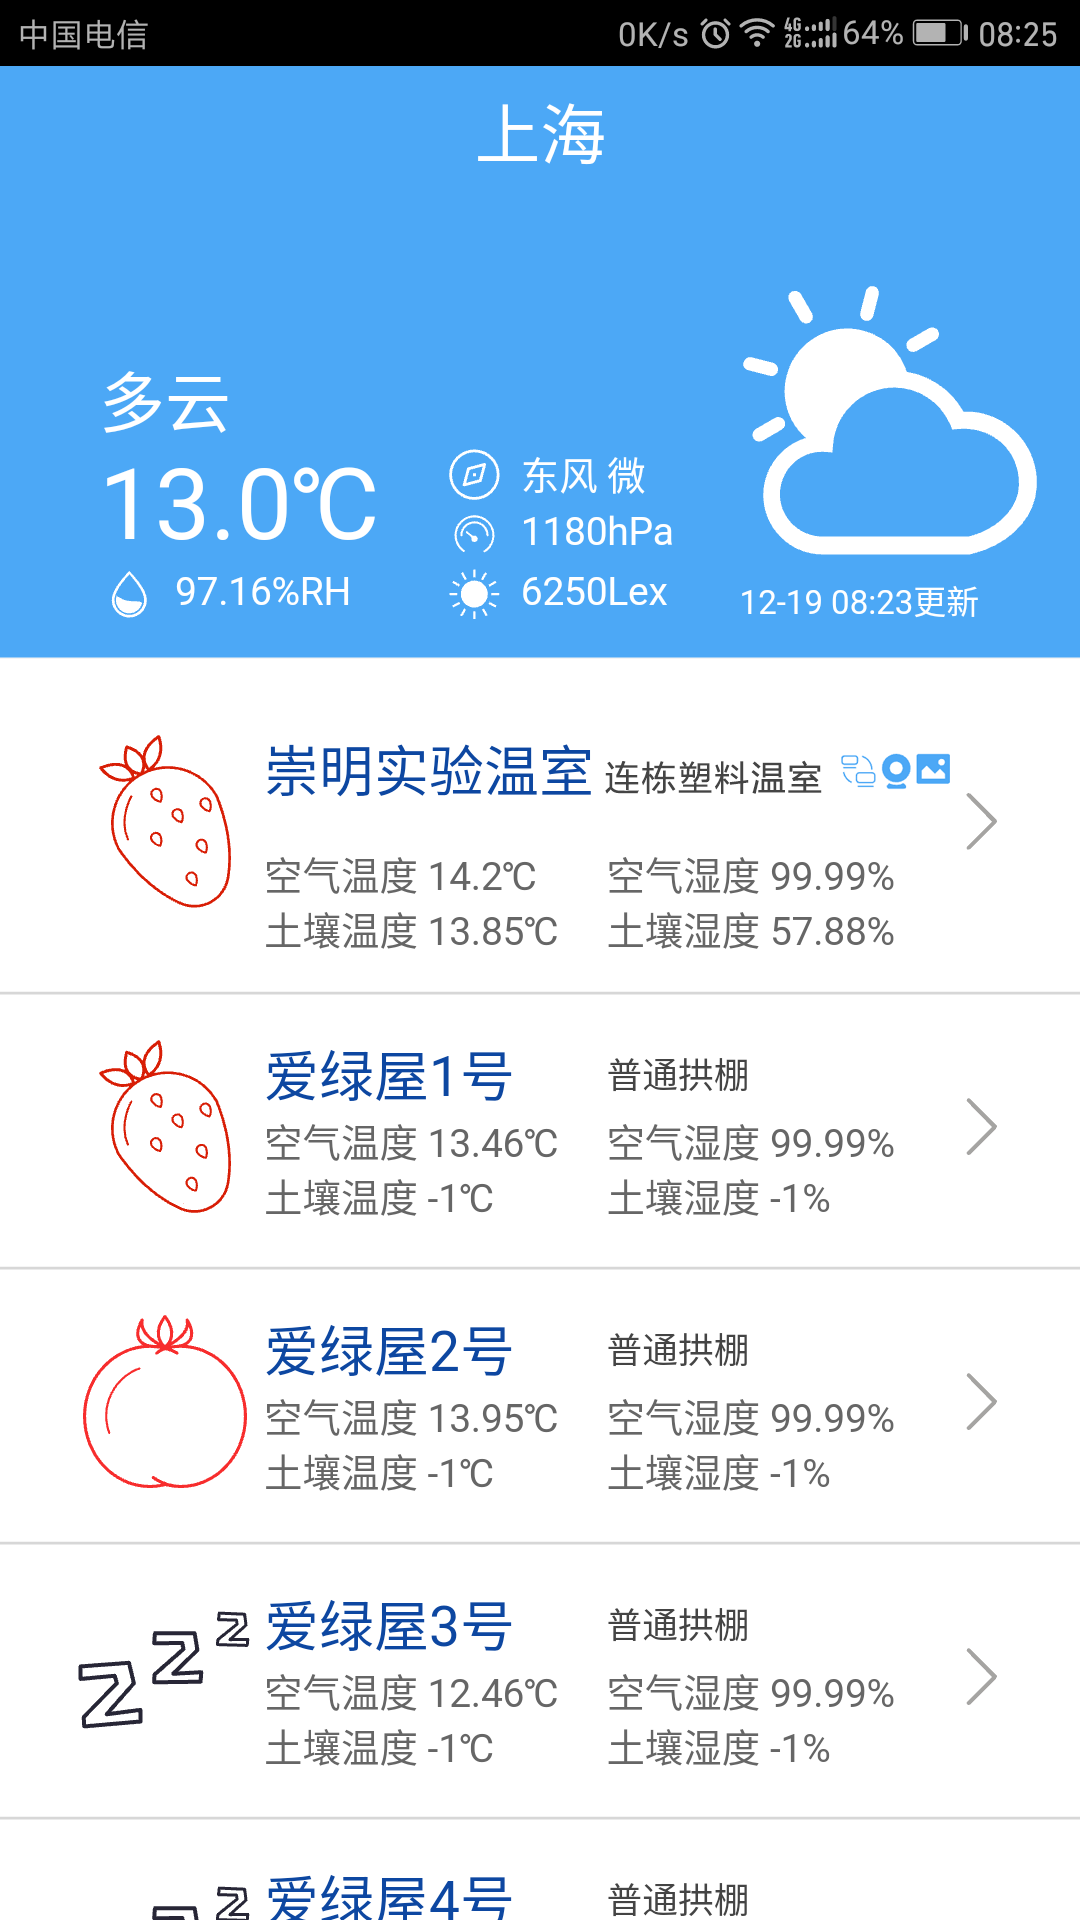
\includegraphics[width=0.19\textwidth]{android/home.png}
		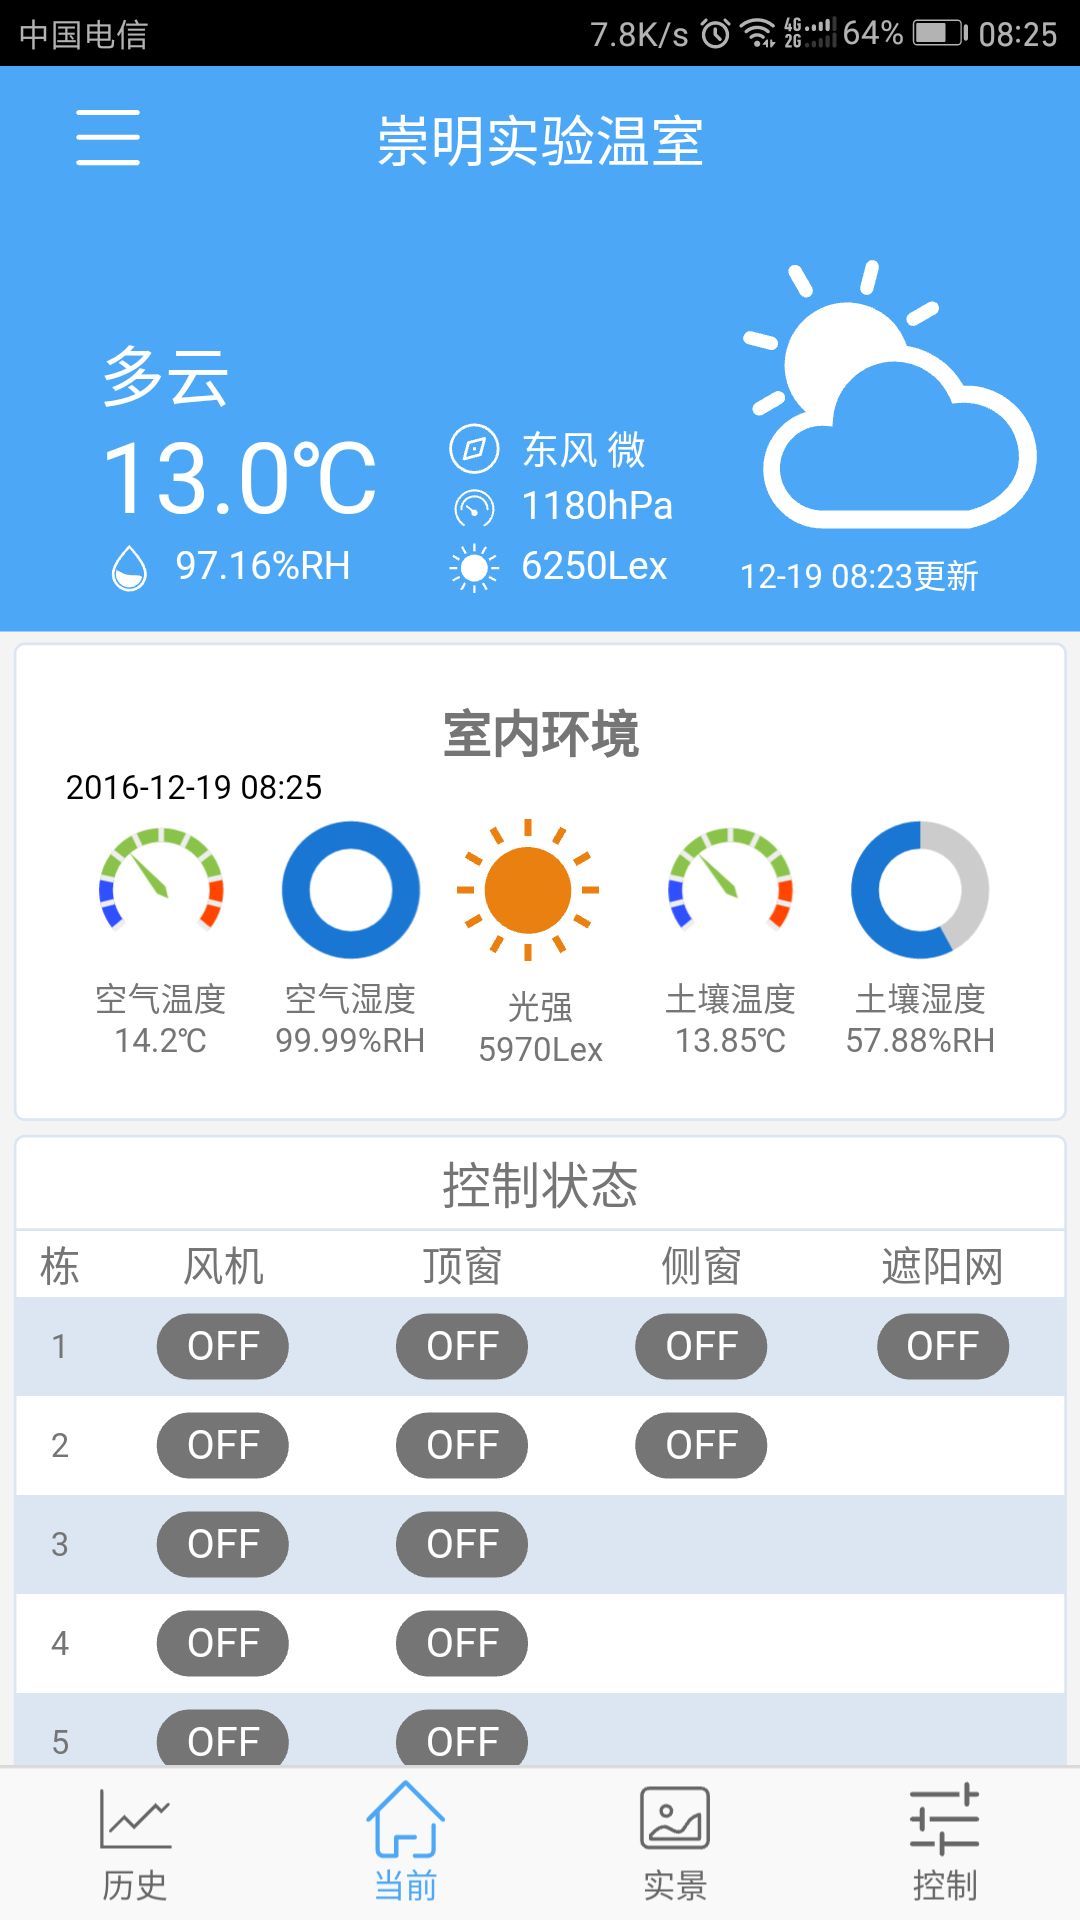
\includegraphics[width=0.19\textwidth]{android/detail.png}
		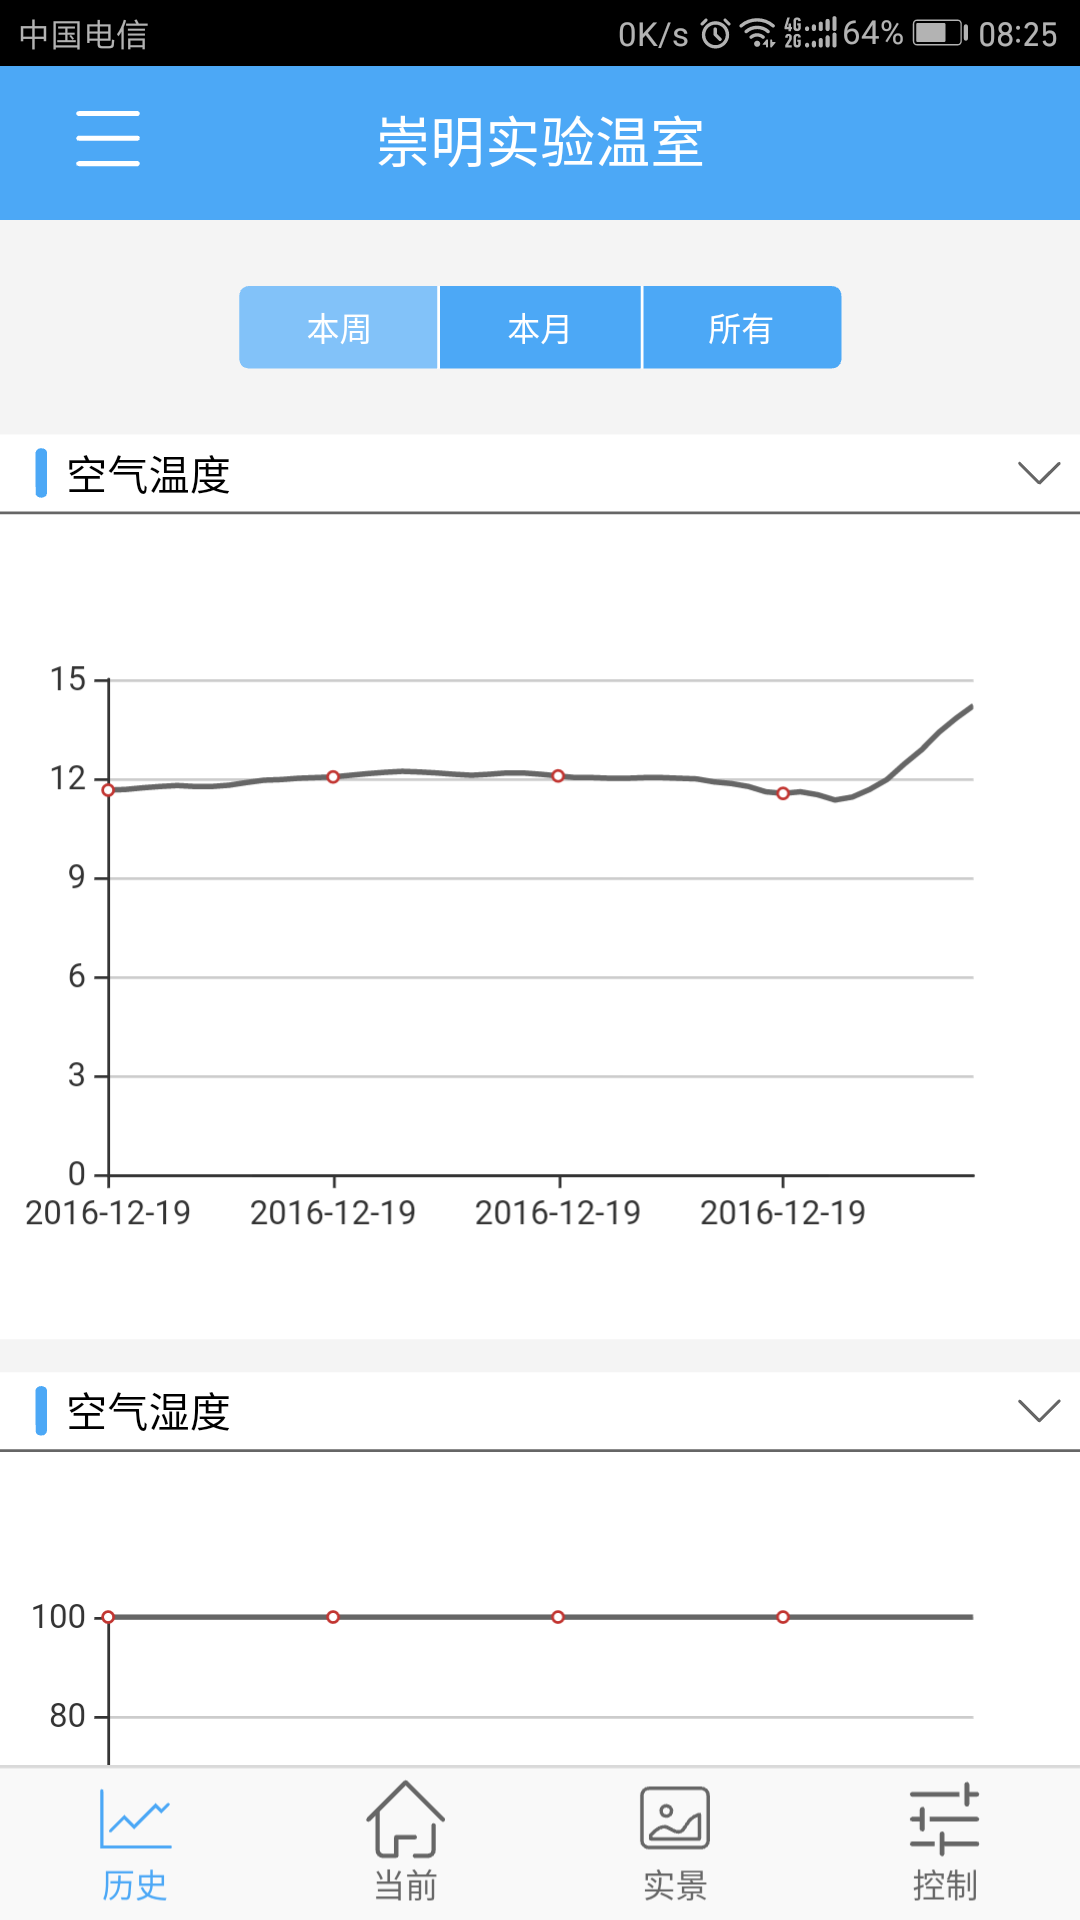
\includegraphics[width=0.19\textwidth]{android/history.png}
		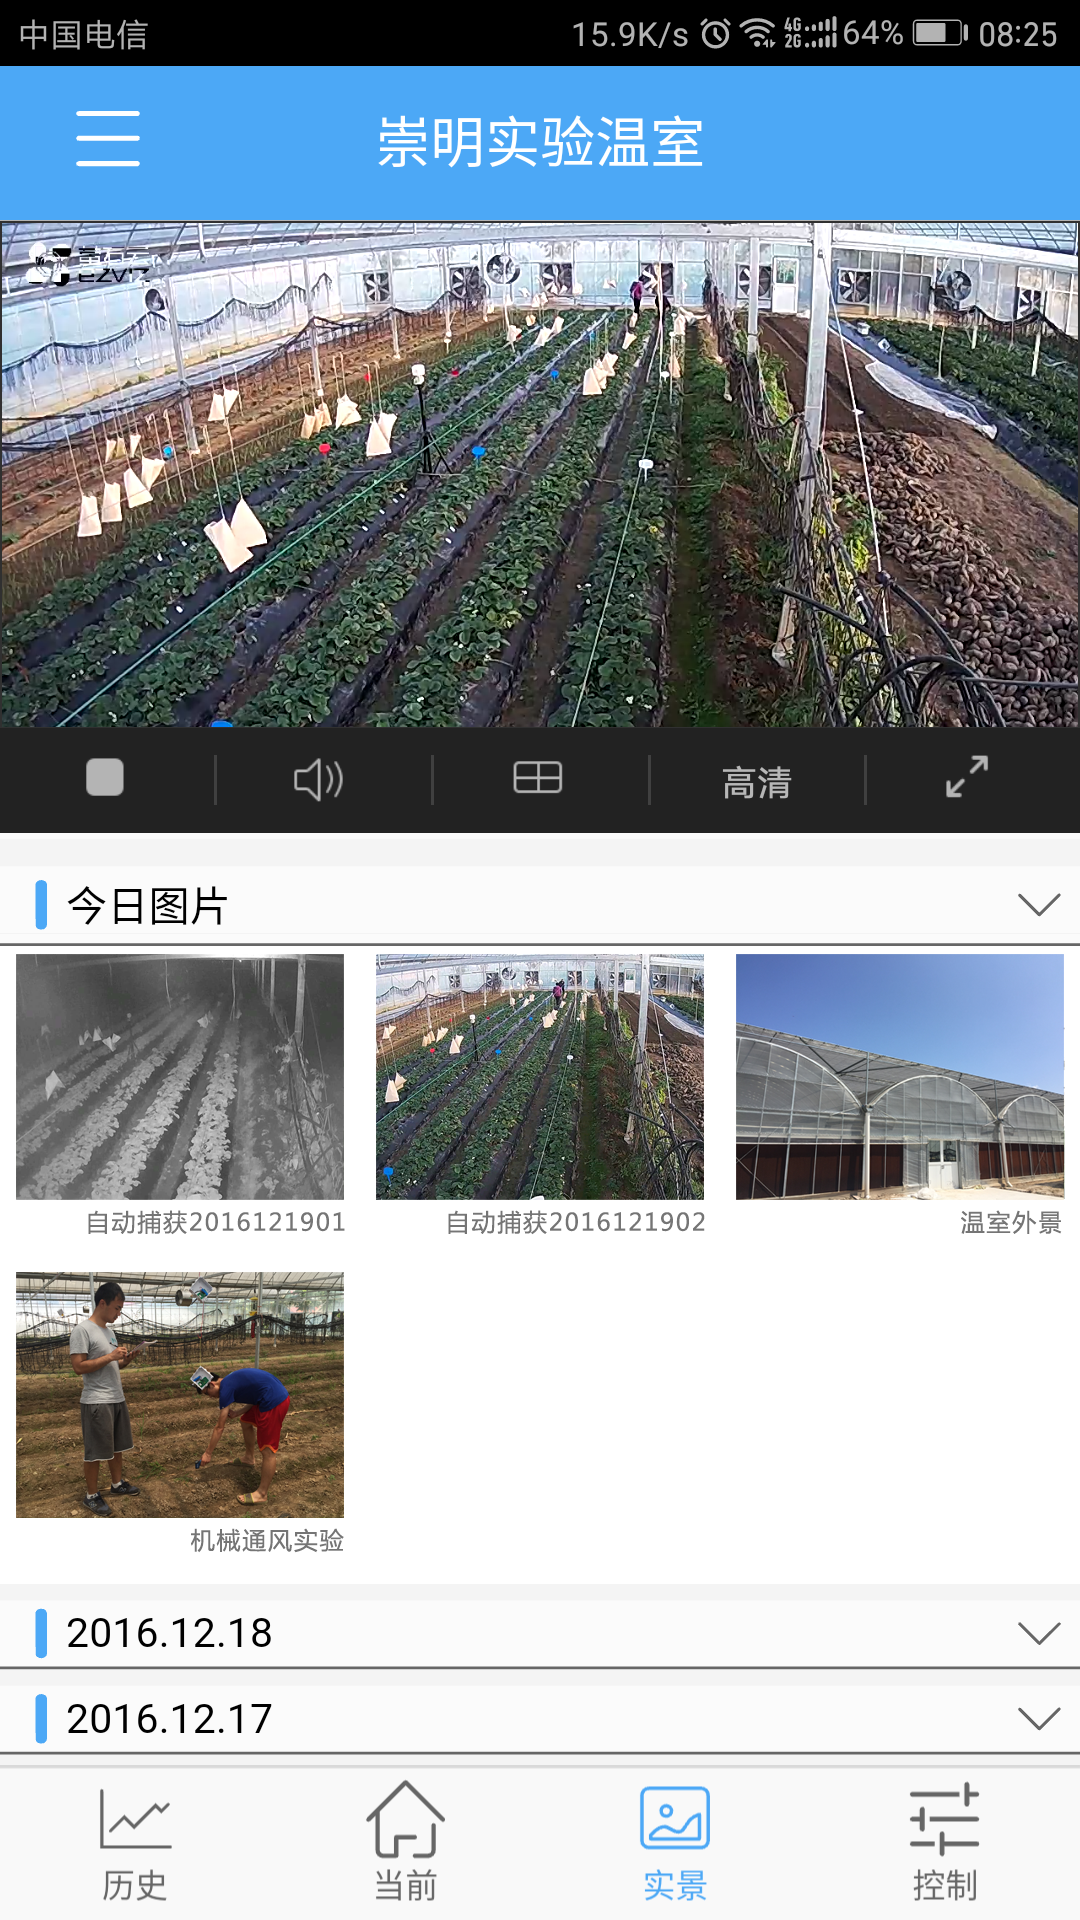
\includegraphics[width=0.19\textwidth]{android/video.png}
		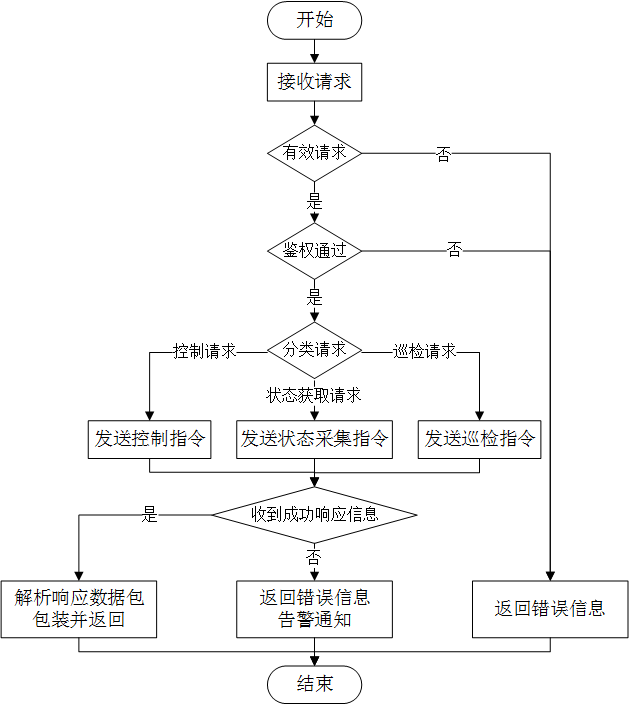
\includegraphics[width=0.19\textwidth]{android/control.png}	
	    \bicaption[fig:snapshot]{终端程序截图}{终端程序截图}{Fig}{Snapshots of the terminal program}
	\end{figure}
现场测试运行结果表明,系统整体稳定可靠,符合预期设计要求和生产要求,可有效提高温室生产过程的科学管理水平。

\section{机械通风优化设计}
	\subsection{机械通风参数优化}
本文主要分析开启风机个数、入口温度、温室长度和环境温度变化(即相对于表\ref{tab:basicParameters}室内地面温度、薄膜壁面温度和薄膜顶棚温度变化)对于温室机械通风降温效果的影响。为分析这些因素的影响,本文控制不同因素变量的变化,共进行了12组仿真计算,各组的参数设置如表\ref{tab:cases}所示,其它基本参数每组保持不变,详情如表\ref{tab:basicParameters}所示。

		\begin{table}[!htbp]
  			\centering
  			\bicaption[tab:cases]{仿真方案参数设置}{仿真方案参数设置}{Table}{Parameters in different simulation cases}
  			\begin{tabular}{ccccc} \toprule
			方案编号 & 风机数量/个 & 入口温度/℃ & 温室长度/m & 环境温度变化/℃\\ \midrule
			1 & 10	 & 30 & 32 & 0\\
			2 & 6 & 30 & 32 & 0\\
			3 & 4 & 30 & 32 & 0\\
			4 & 2 & 30 & 32 & 0\\
			5 & 10 & 28 & 32 & 0\\
			6 & 10 & 29 & 32 & 0\\
			7 & 10 & 31 & 32 & 0\\
			8 & 10 & 30 & 40 & 0\\
			9 & 10 & 30 & 48 & 0\\
			10 & 10 & 30 & 100 & 0\\
			11 & 10 & 30 & 32 & 1\\
			12 & 10 & 30 & 32 & -1\\ \bottomrule
 			\end{tabular}
		\end{table}
	如图\ref{fig:cases}所示为不同仿真方案下,植物冠层即截面L空气温度仿真平均值的变化曲线。
	
		\begin{figure}[!htbp]
		\centering
		\subfigure[不同风机开启情况]{
			\label{fig:cases:a}
			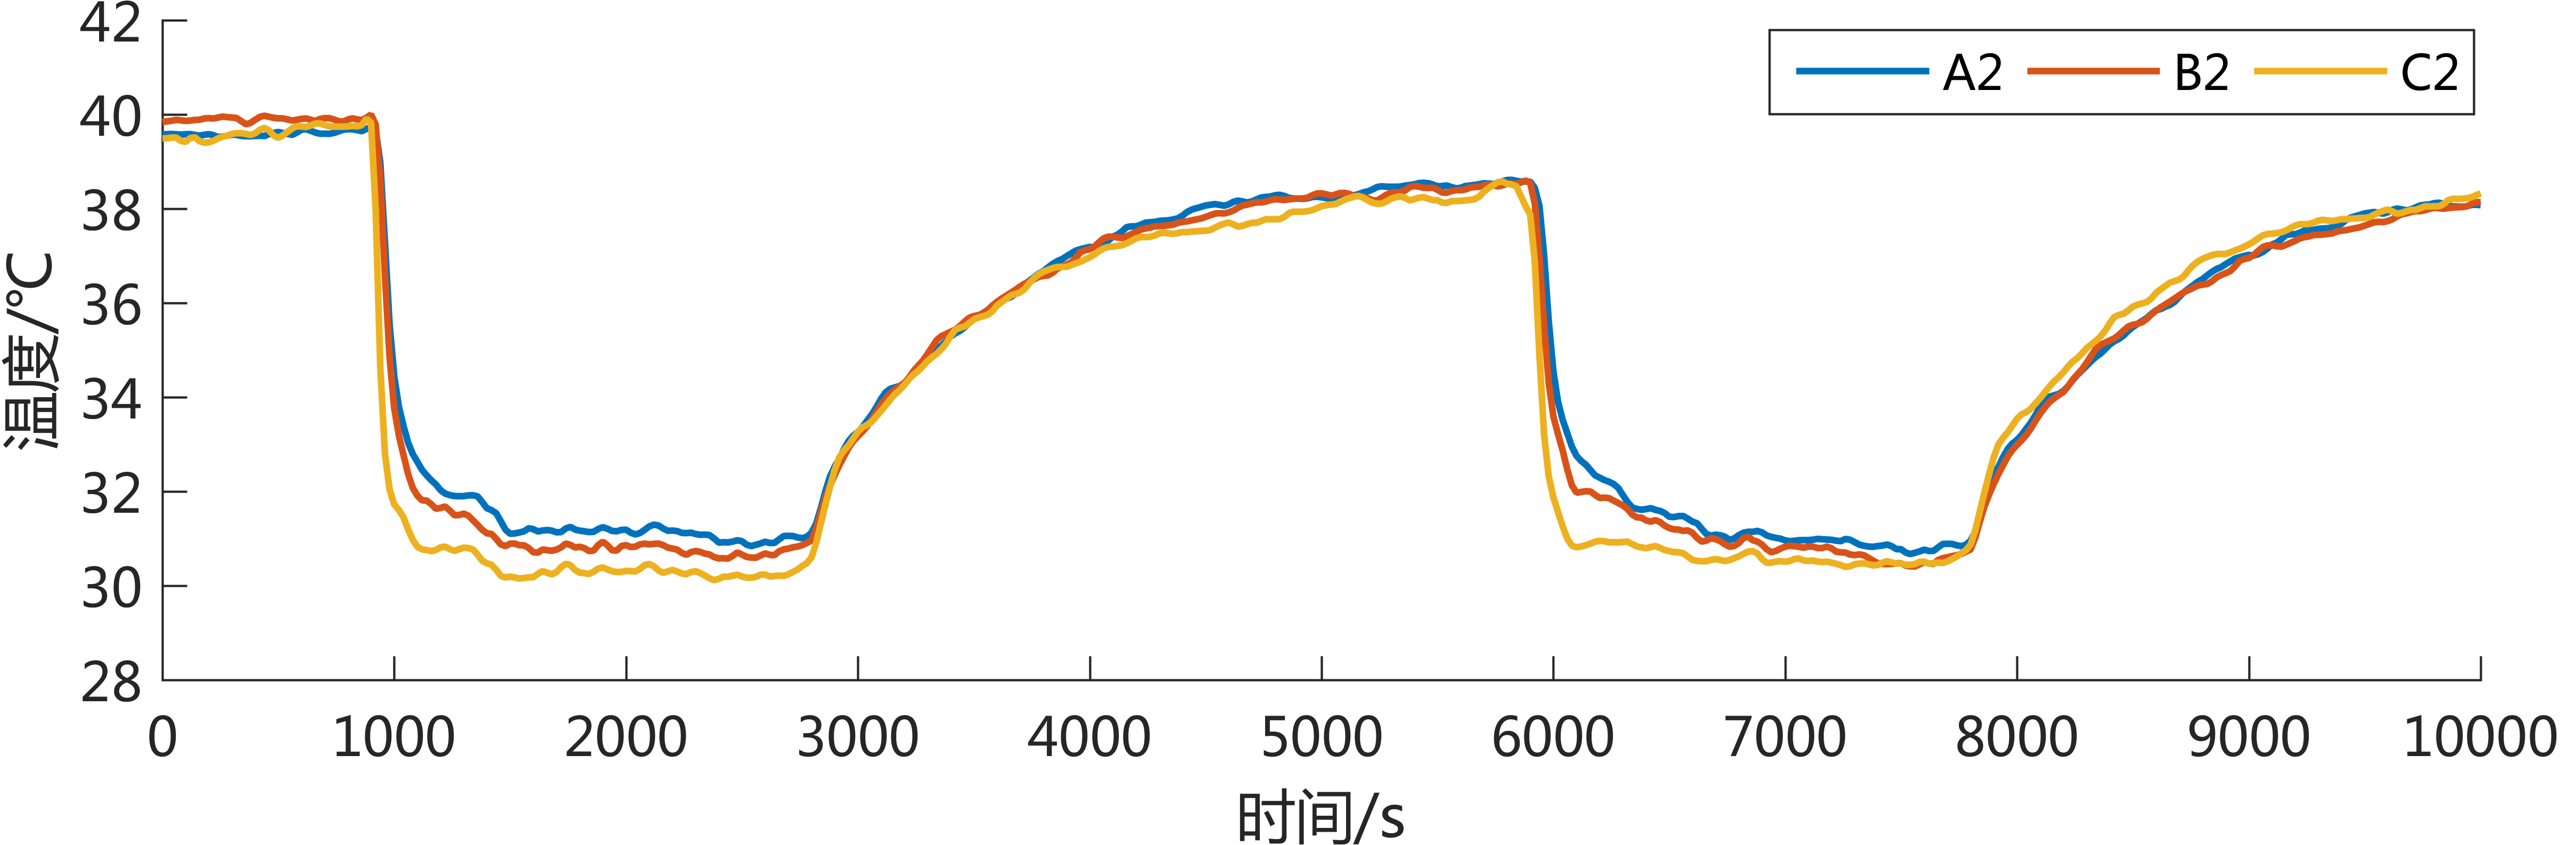
\includegraphics[width=0.4\textwidth]{cases/01.png}
		}
		\subfigure[不同温室长度]{
			\label{fig:cases:b}
			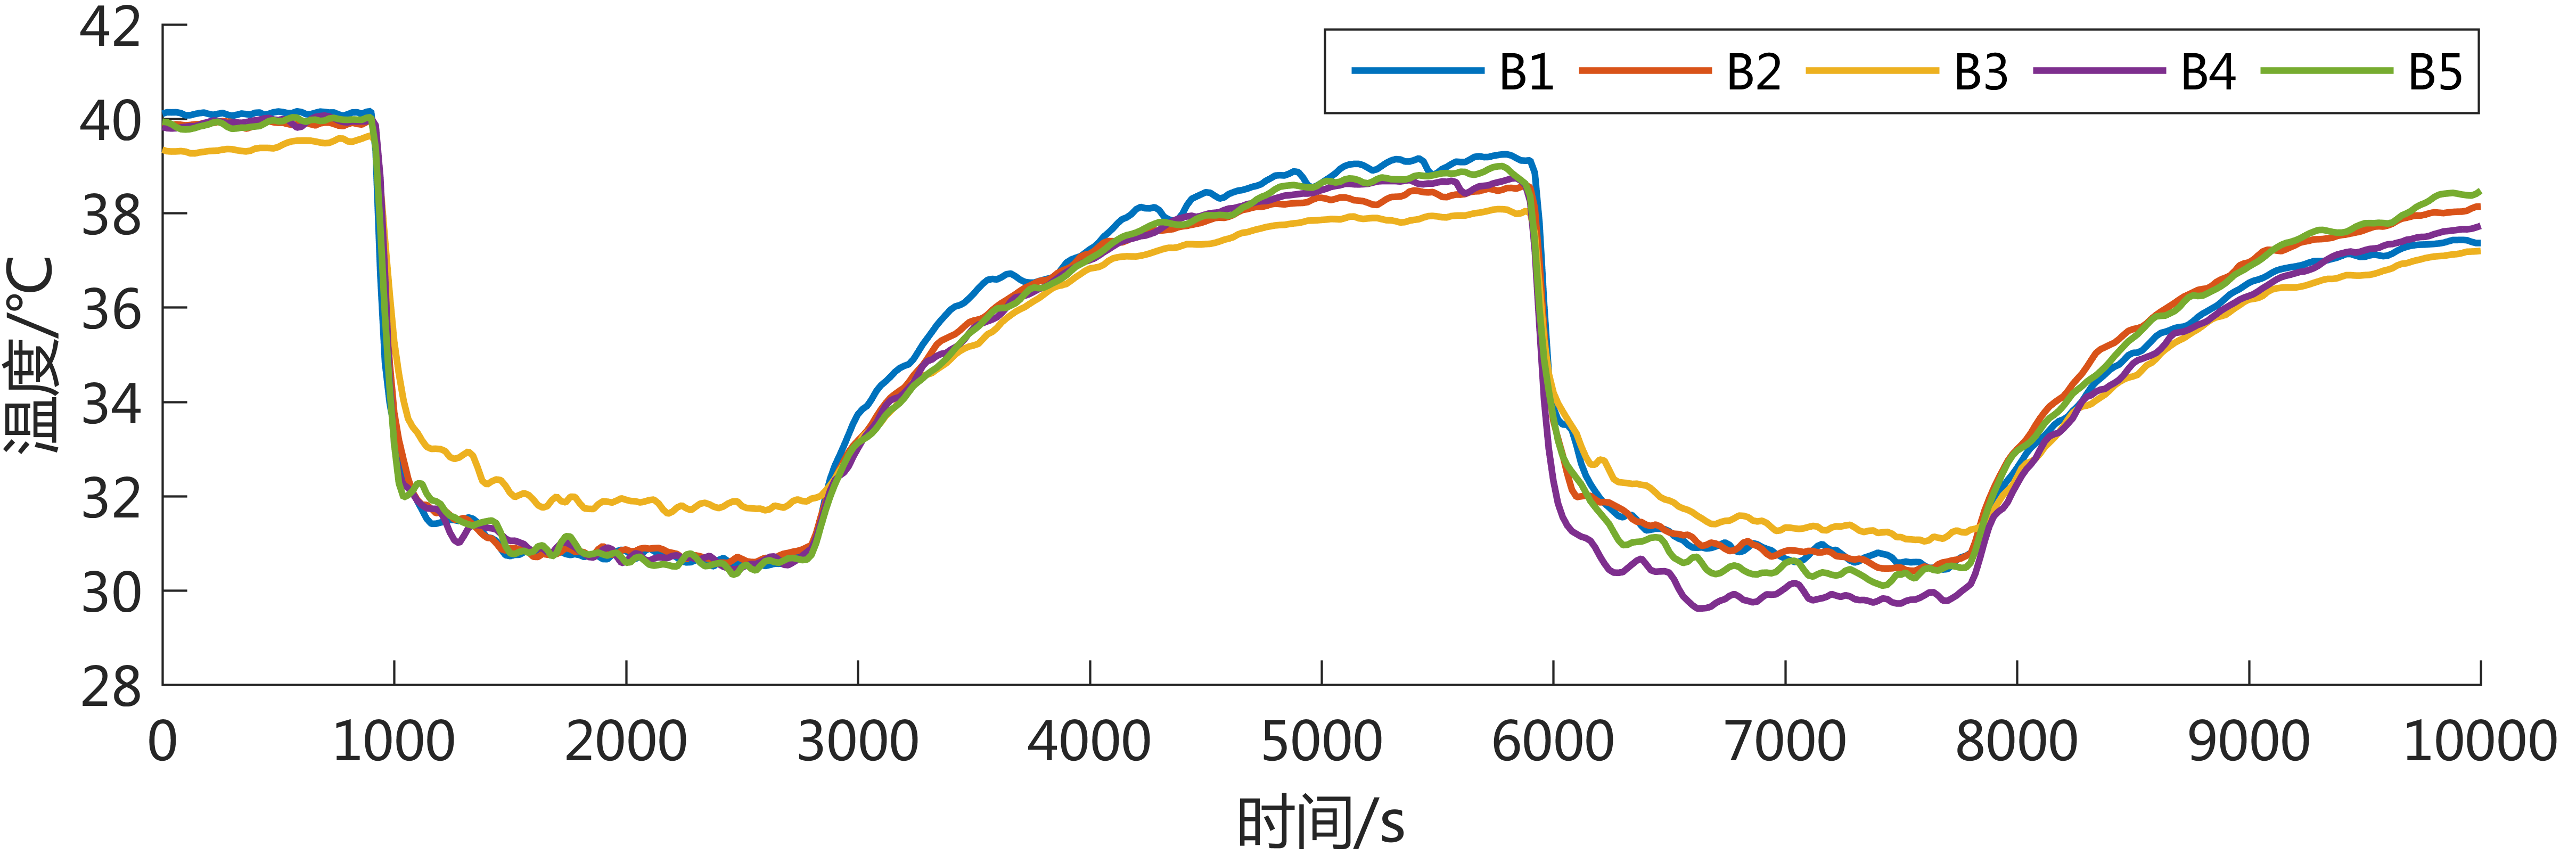
\includegraphics[width=0.4\textwidth]{cases/02.png}
		}
		\subfigure[不同入口温度]{
			\label{fig:cases:c}
			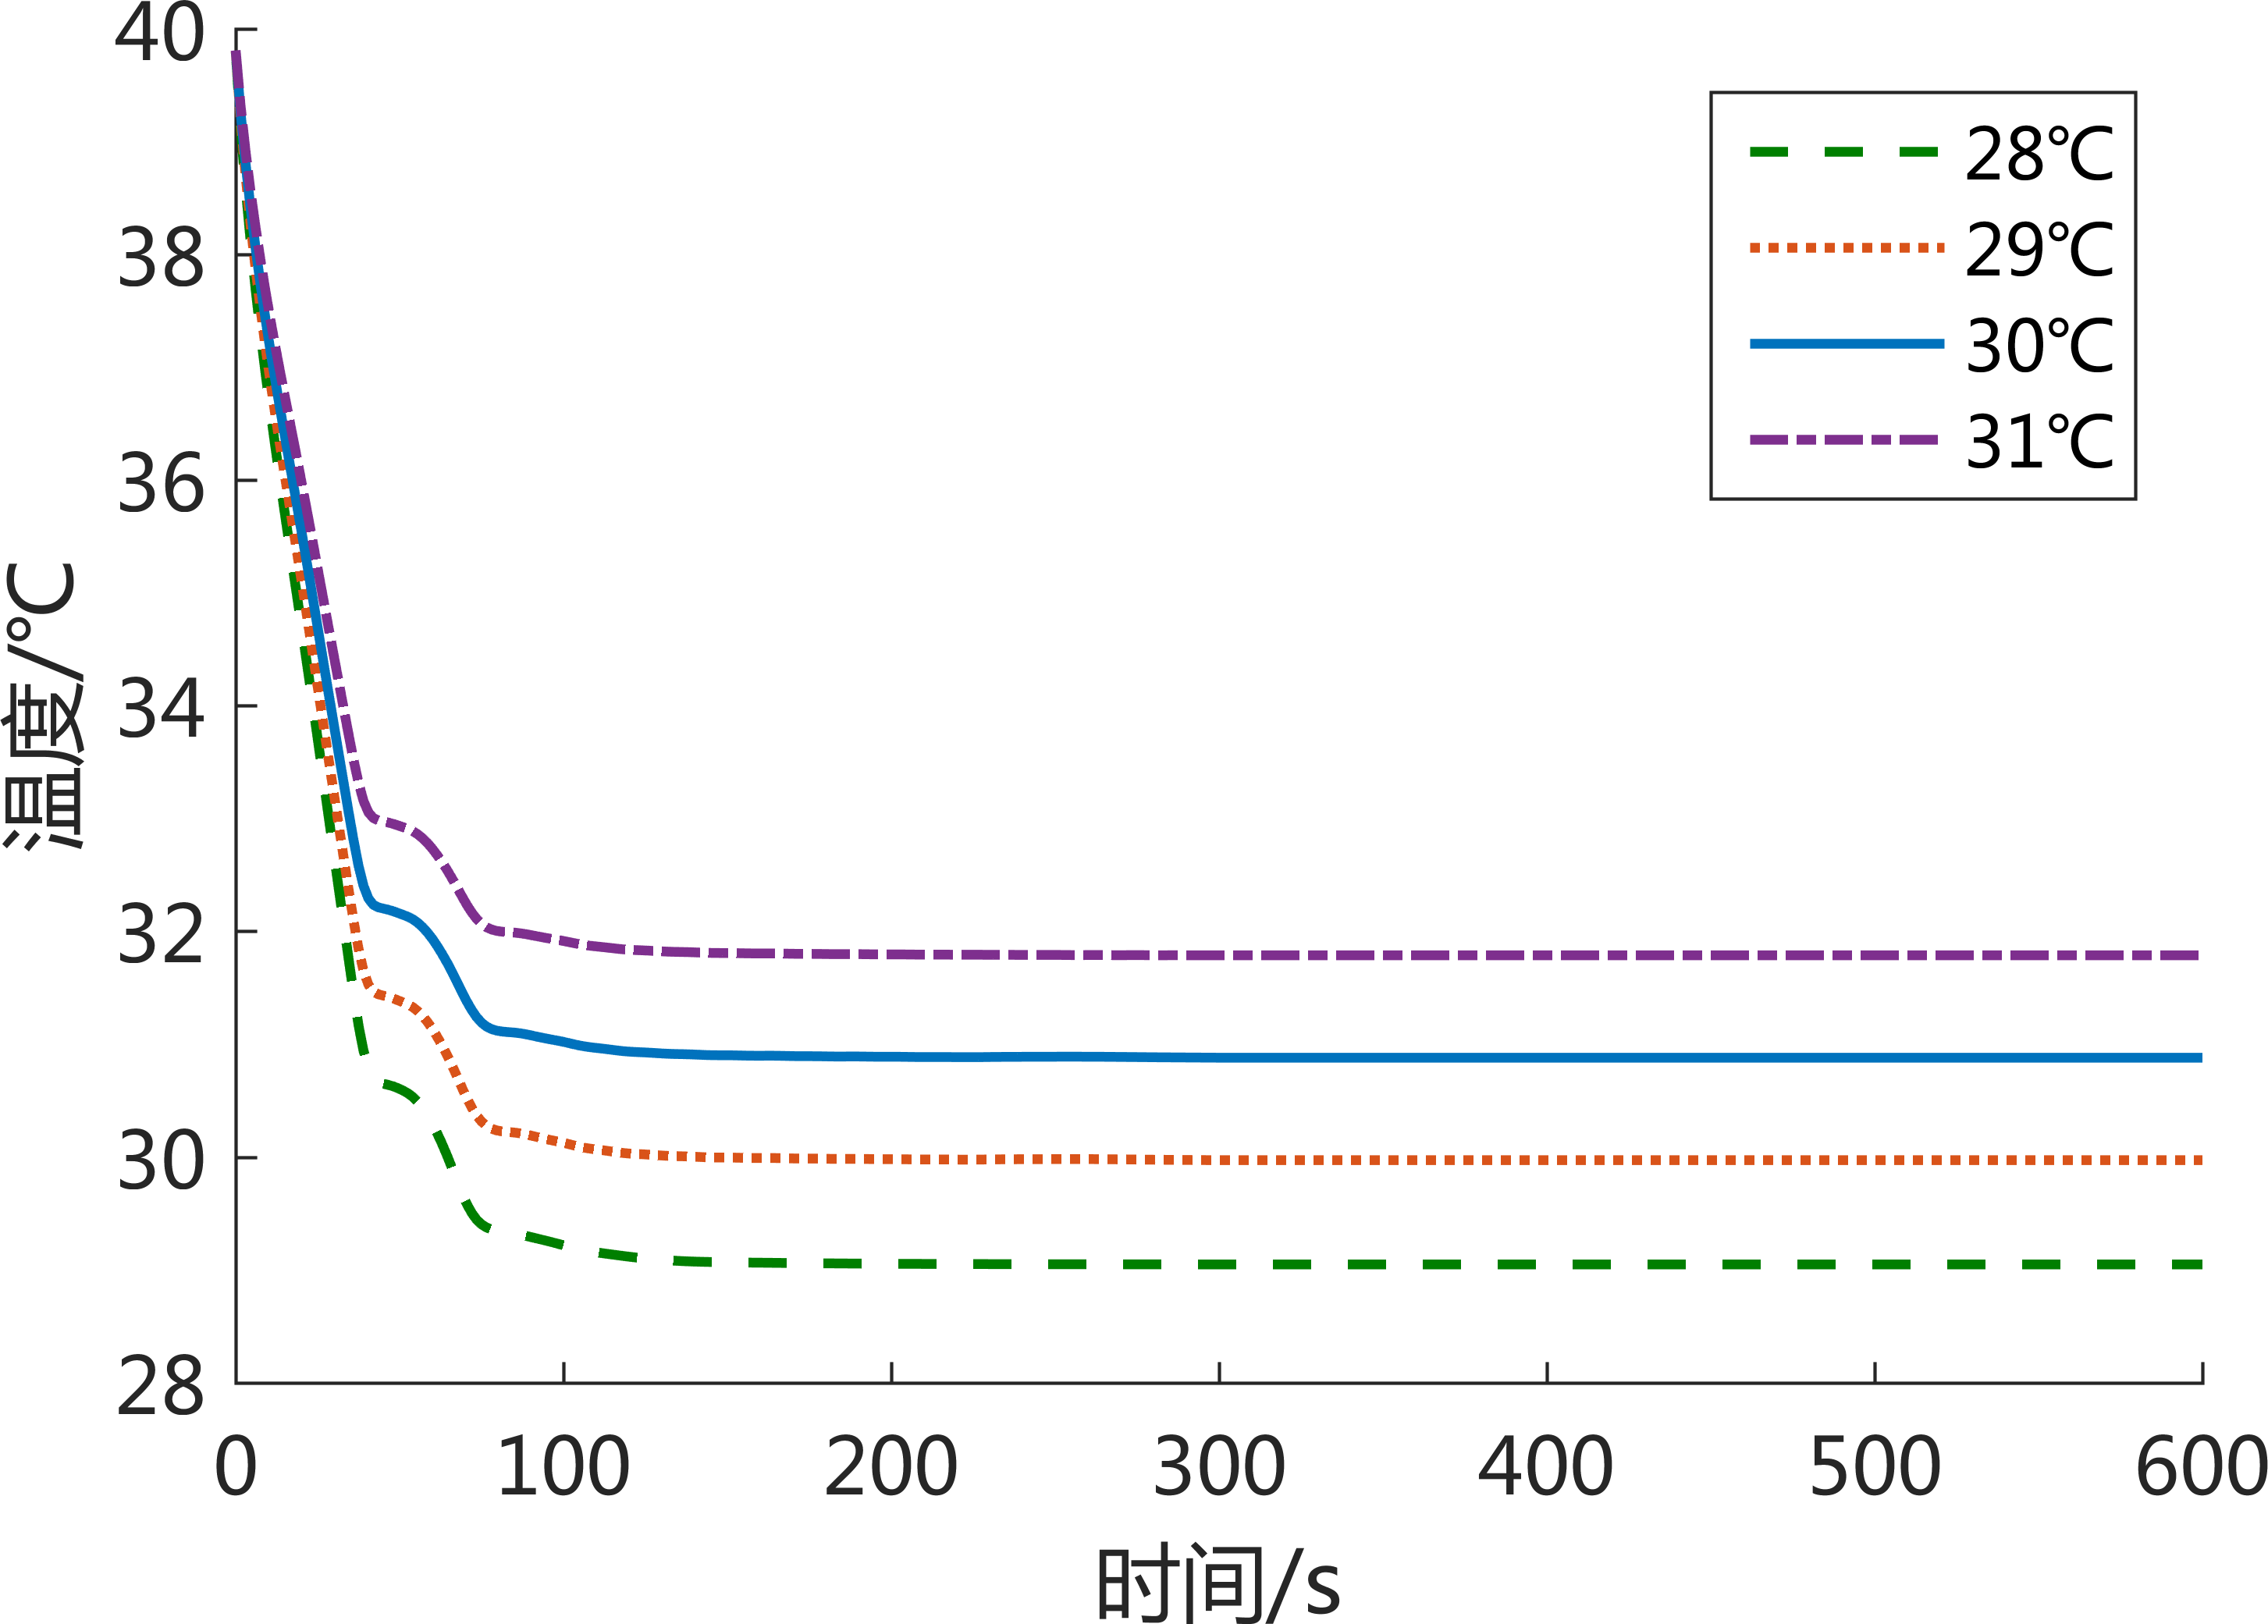
\includegraphics[width=0.4\textwidth]{cases/03.png}
		}
		\subfigure[不同环境温度变化]{
			\label{fig:cases:d}
			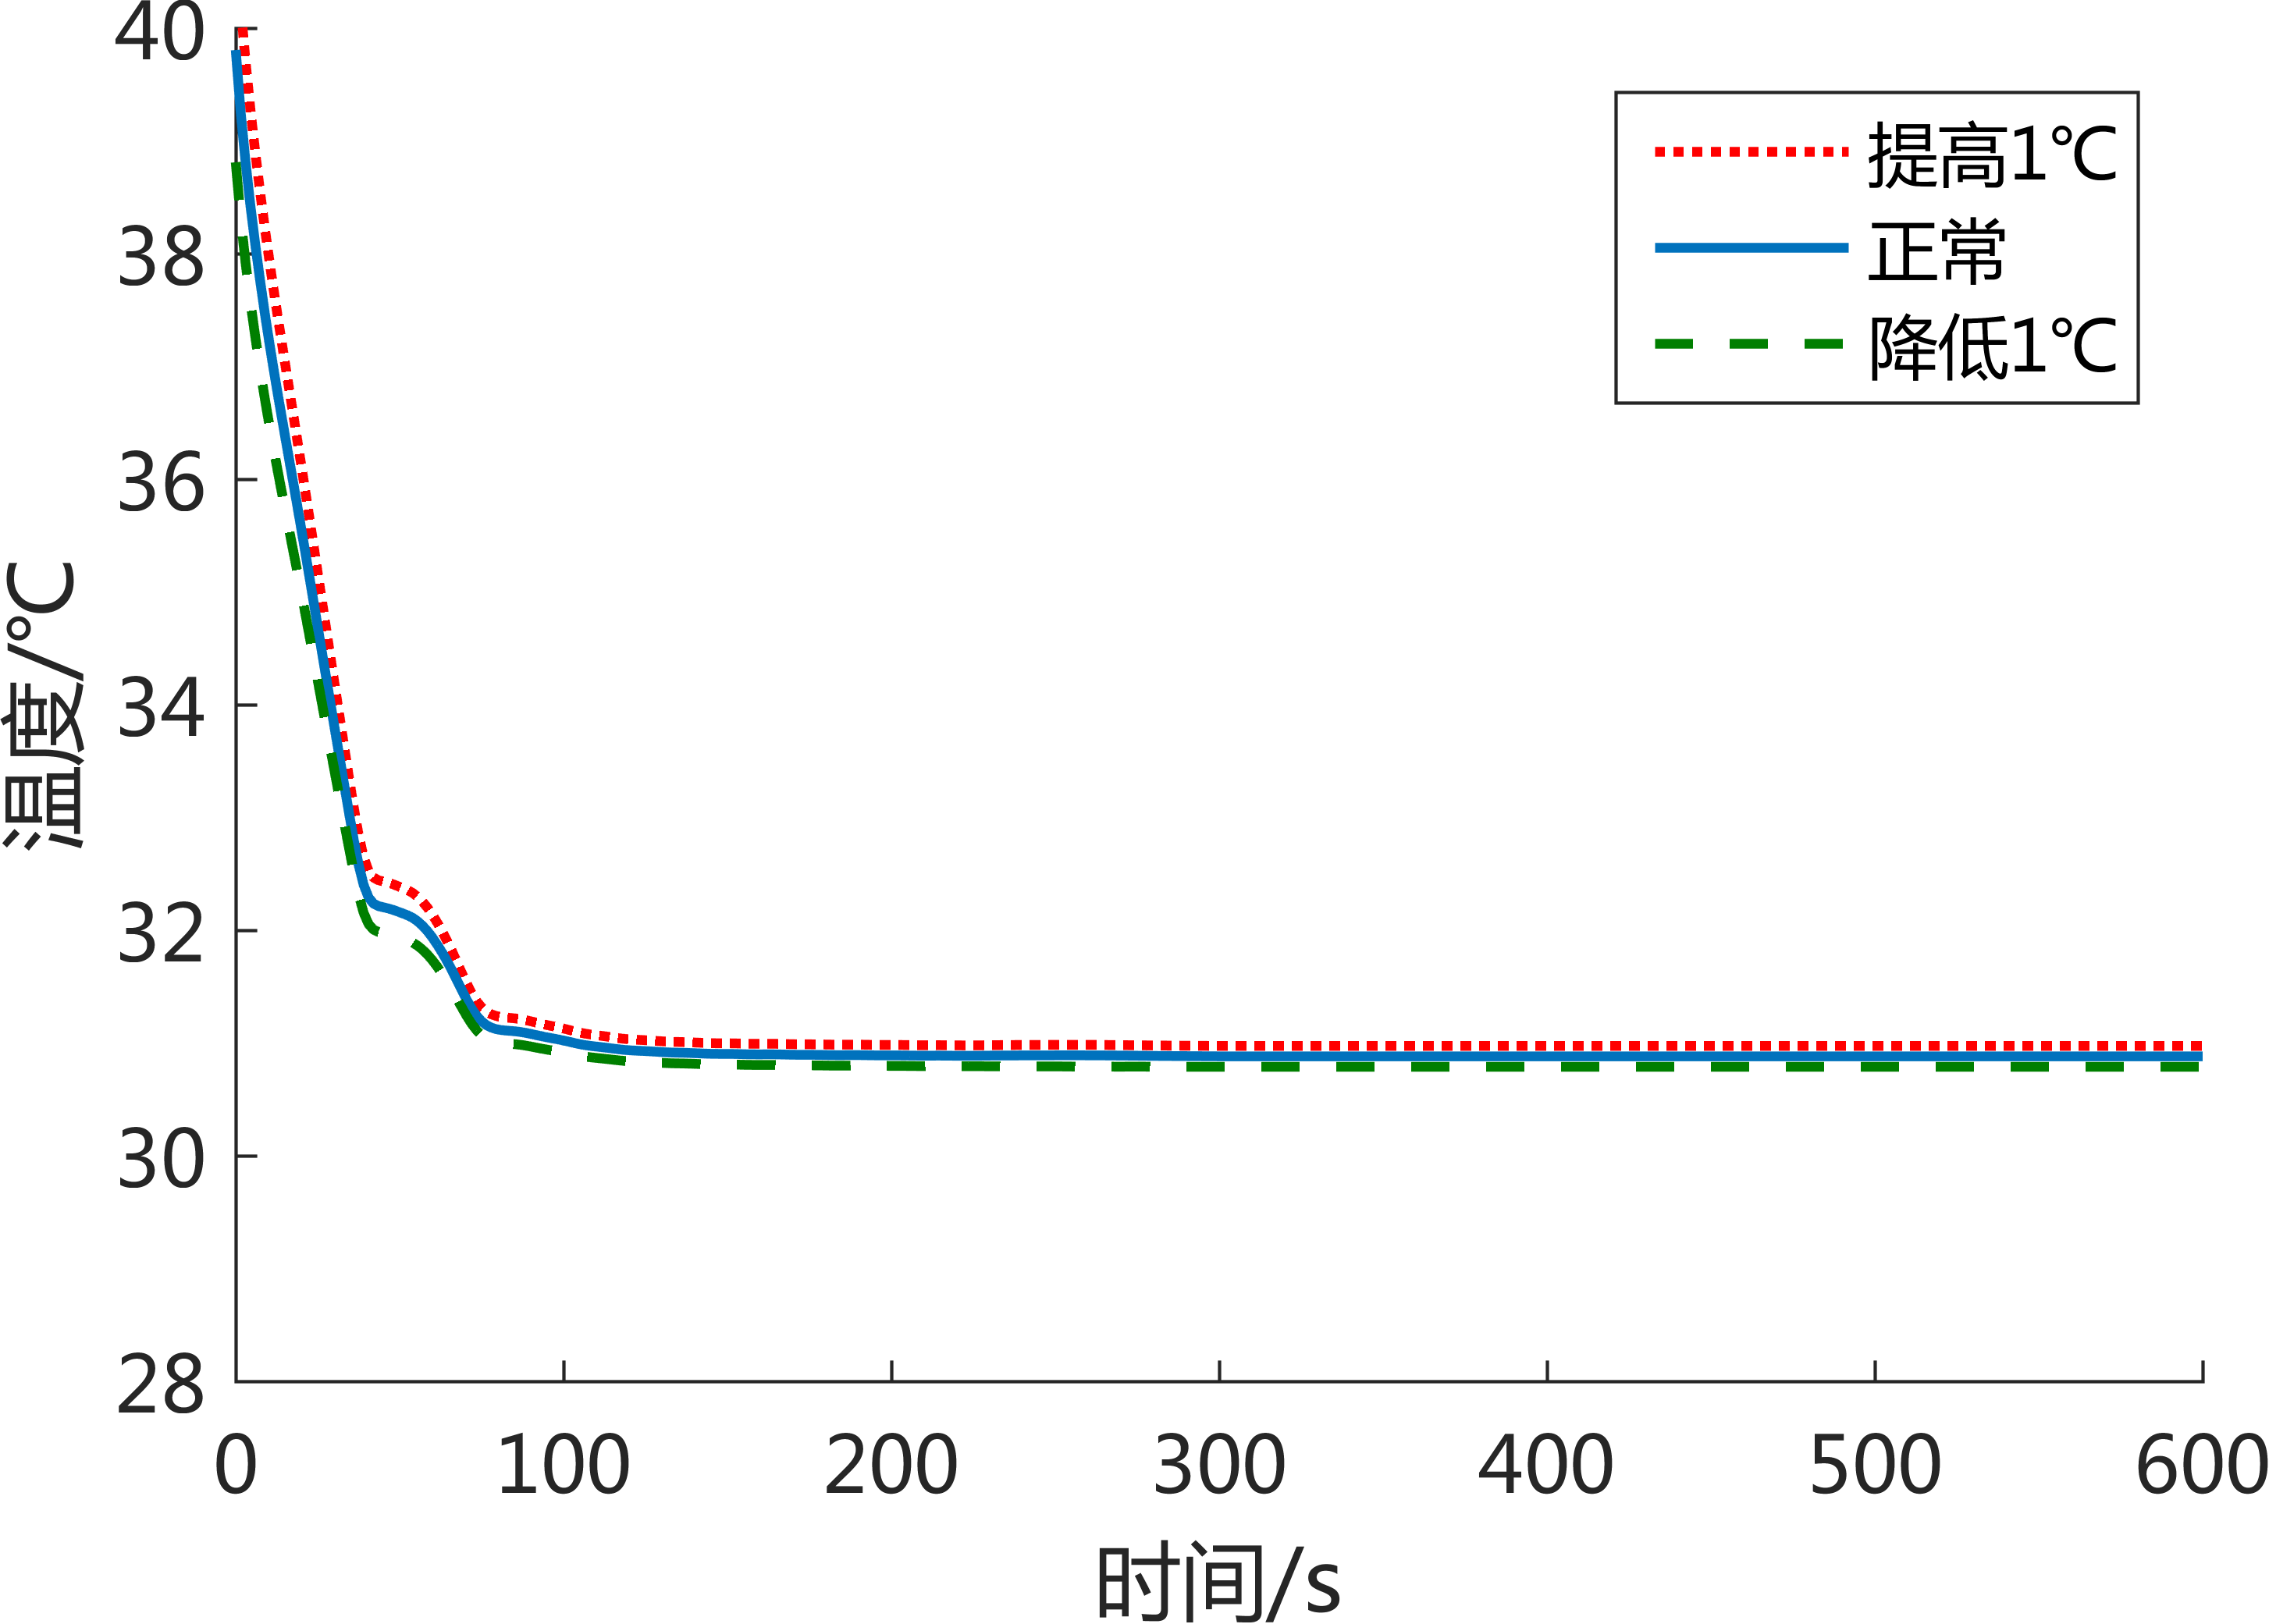
\includegraphics[width=0.4\textwidth]{cases/04.png}
		}
 		\bicaption[fig:cases]{截面L不同方案下空气温度仿真平均值变化曲线}{截面L不同方案下空气温度仿真平均值变化曲线}{Fig}{Simulated average values of air temperature in different cases at section L}
 	\end{figure}
由图\ref{fig:cases:a}可以看出开启风机数量对于温室内降温速度的影响较大,但是在一定范围内对于温室最终的稳定温度影响较小。随着开启风机数量的减少,温室内降温速度在一定程度上变慢,且稳定温度会略微升高。相较于开启10台风机时降温至稳定温度的时间,开启6台风机时约为其1.5倍,开启4台风机时约为其2.2倍,开启2台风机时约为其4.5倍。相较于开启10台风机时最终降温的稳定温度,开启6台风机时和4台风机时约升高0.3℃,开启2台风机时约升高0.7℃。根据这一现象,可以对温室机械通风设计时风机的配置和运行时开启风机的数量可以进行一定的优化,即在对降温速度要求不高的情况下,可适当减少风机的配置数量或开启风机的数量,降低机械通风硬件成本,同时可以降低运行成本和减少能耗;对于种植对温度较为敏感的作物的温室,可以在温度上升到过高之前提前开启风机,此时也可适当减少运行风机的数量达到相同的降温效果。

由图\ref{fig:cases:b}可以看出,温室长度的增加会影响降温效果,不仅会增加降温时间,而且会提高稳定温度,但在一定范围内对降温效果的影响较小,对于降温时间的增加和稳定温度的提高都不是很明显,如仿真结果显示在温室长度增加50\%,即由32 m增加到48 m的情况下,最终可降低到的平均稳定温度仅升高约0.5℃,但此时单位面积上的机械通风能耗明显下降。根据这一现象,可以在温室设计之初对温室结构参数进行一定的优化,即在作物对温度不是特别敏感的情况下,可适当增加温室的长度,降低温室单位面积的机械通风能耗。

由图\ref{fig:cases:c}可以看出,入口温度的降低对于降温速度的影响较小,但会显著影响温室降温最终可以达到的稳定温度。随着湿帘处入口温度的降低,稳定温度会随之明显降低,由仿真结果可知入口温度每降低1℃,稳定温度平均可降低0.9℃。根据这一现象可知,入口温度对于温室降温效果的影响较为显著,因此可通过降低入口温度的方式改善降温效果,一般情况下可以使用如抽取地下水浸湿湿帘、增加湿帘厚度等方式降低入口温度。

由图\ref{fig:cases:d}可以看出,外界环境温度较小范围的改变,对于机械通风的降温效果影响较小。

	\subsection{机械通风策略优化}
图\ref{fig:strategy}所示为不同控制策略下,植物冠层即截面L空气温度仿真平均值的变化曲线。策略1为开启10台风机持续工作;策略2为开启10台风机降温至稳态温度后关闭风机,待温度回升到一定程度后再次开启10台风机降温,为保证温室平均气温低于32℃,本文在温度回升至32.59℃时即再次开启风机进行降温;策略3为开启10台风机迅速降温至稳态温度后只保留4台风机开启维持降温效果。

	\begin{figure}[!htbp]
		\centering
		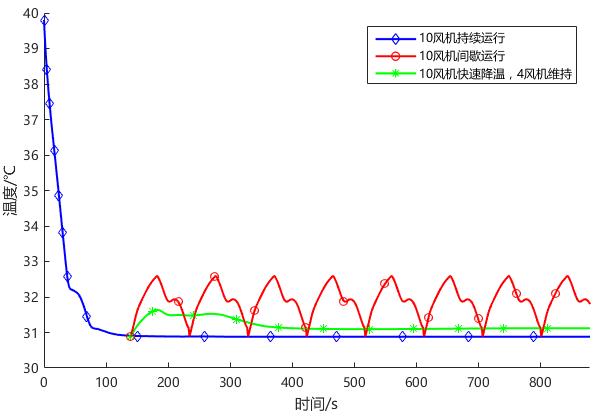
\includegraphics[width=0.7\textwidth]{strategy.png}
		\bicaption[fig:strategy]{截面L不同控制策略下空气温度仿真平均值变化曲线}{截面L不同控制策略下空气温度仿真平均值变化曲线}{Fig}{Simulated average values of air temperature with different control strategies at section L}
	\end{figure}
	在长时间连续降温的过程中,开始阶段的快速降温的能耗可忽略,因此选取稳定阶段,即600 s以后的两个完整周期评价不同控制策略的效果,结果如表\ref{tab:strategies}所示。
	
		\begin{table}[!htbp]
			\bicaption[tab:strategies]{不同控制策略结果比较}{不同控制策略结果比较}{Table}{Comparison of results with different control strategies}
  			\centering
  			\begin{threeparttable}[b]
  			\begin{tabular}{cccc} \toprule
			参数 & 策略1 & 策略2 & 策略3\\ \midrule
			风机数量/个 & 10 & 10 & 4\\
			间歇比\tnote{1} & 1 & 0.53 & 1\\
			等效风机数量/个 & 10 & 5.3 & 4\\
			平均温度/℃ & 30.88 & 31.82 & 31.09\\
			最高温度/℃ & 30.88 & 32.59 & 31.09\\
			温度稳定性\tnote{2} \hspace{1mm} /℃ & <0.1 & <0.43 & <0.1\\ \bottomrule
 			\end{tabular}
 			\begin{tablenotes}
    			\item [1] 风机开启时间的占比。
    			\item [2] 完整周期内的温度均方根误差。
   			 \end{tablenotes}
  		\end{threeparttable}
		\end{table}
	由控制策略结果比较表可知:
	
策略1的降温效果和稳定性都是最好的,但是大量风机连续工作导致能源消耗过大,降温成本较高。

策略2温室的降温效果较差,和策略1相比平均温度升高0.94℃,稳定性也较差,但相较于策略1可降低约47\%的能源消耗。

策略3温室的降温效果略微变差,和策略1相比平均温度仅升高0.21℃,稳定性也较好,同时相较于策略1可降低60\%的能源消耗。

因此针对实验温室,选择策略2和策略3都能大幅降低能源消耗,而策略3从实现的简单和效果两方面都为较适宜的机械通风控制策略。

\section{本章小结}
本章首先通过对经过验证的温室CFD仿真模型的仿真结果进行分析,得到了针对实验温室在高温条件下需要机械通风情况下的监测点位置选择与优化方案。然后对本文设计并实现的基于农业物联网的智能温室监测与控制系统在实验温室内进行了实践与应用,并得到了良好的使用效果,验证了系统的稳定性和可靠性。最后,针对实验温室,通过仿真模型模拟了室外高温条件下的风机数量、温室长度、入口温度及环境温度变化等参数对机械通风降温效果的影响程度,并模拟了不同数量风机启闭控制的降温效果,为温室结构参数和通风设备配置的优化提供了参考,为控制系统提供了优化的夏季机械通风降温控制策略。该部分优化方案虽然针对实验温室进行,但是仍可为其它同类温室机械通风系统的优化设计和节能减排提供一定的参考。
